\documentclass[a4paper,10pt]{article}
\usepackage[utf8]{inputenc}
 
% Blank line between paragraphs instead of indenting the first line
\usepackage{parskip}
\setlength{\parskip}{\baselineskip}

% Squash a bit more text onto a page
\usepackage{geometry}
\geometry{verbose,tmargin=20mm,bmargin=20mm,lmargin=25mm,rmargin=25mm}

\usepackage{graphicx}
\usepackage{listings}
\usepackage{amsmath}
\usepackage{verbatim}
\usepackage{xcolor}

% Indent verbatim environments
\makeatletter \def\verbatim@processline{\hspace*{2em}\the\verbatim@line\par}\makeatother

\lstdefinelanguage{logicdef}
{
  morekeywords={DEVICES, MONITORS, CONNECTIONS, END},
  sensitive=false,
  morecomment=[s]{/*}{*/},
  basicstyle=\small\ttfamily,
  keywordstyle=\pmb,
  frame=single,
  numbers=left,
  numberstyle=\tiny
}

\definecolor{darkgreen}{rgb}{0,0.7,0}
\definecolor{darkred}{rgb}{0.7,0,0}

\lstdefinelanguage{diff}
{
  morecomment=[f][\color{blue}]{@@},     % group identifier
  morecomment=[f][\color{darkred}]{-},         % deleted lines 
  morecomment=[f][\color{darkgreen}]{+},       % added lines
  morecomment=[f][\color{magenta}]{---}, % Diff header lines (must appear after +,-)
  morecomment=[f][\color{magenta}]{+++},
  basicstyle=\small\ttfamily,
  breakatwhitespace=false,         % sets if automatic breaks should only happen at whitespace
  breaklines=true,                 % sets automatic line breaking
  frame=single,
  numbers=none
}

\definecolor{mygreen}{rgb}{0,0.6,0}
\definecolor{mygray}{rgb}{0.5,0.5,0.5}
\definecolor{mymauve}{rgb}{0.58,0,0.82}

\lstset { 
  backgroundcolor=\color{white},   % choose the background color; you must add \usepackage{color} or \usepackage{xcolor}
  basicstyle=\small\ttfamily,      % the size of the fonts that are used for the code
  breakatwhitespace=false,         % sets if automatic breaks should only happen at whitespace
  breaklines=true,                 % sets automatic line breaking
  captionpos=b,                    % sets the caption-position to bottom
  commentstyle=\color{mygreen},    % comment style
  deletekeywords={...},            % if you want to delete keywords from the given language
  escapeinside={\%*}{*)},          % if you want to add LaTeX within your code
  extendedchars=true,              % lets you use non-ASCII characters; for 8-bits encodings only, does not work with UTF-8
  frame=single,                    % adds a frame around the code
  keepspaces=true,                 % keeps spaces in text, useful for keeping indentation of code (possibly needs columns=flexible)
  columns=flexible,
  keywordstyle=\color{blue},       % keyword style
  language=C++,                    % the language of the code
  morekeywords={*,DEVICES,
  				CONNECTIONS,
  				MONITORS,
  				END}, 	           % if you want to add more keywords to the set
  numbers=left,                    % where to put the line-numbers; possible values are (none, left, right)
  numbersep=5pt,                   % how far the line-numbers are from the code
  numberstyle=\tiny\color{mygray}, % the style that is used for the line-numbers
  rulecolor=\color{black},         % if not set, the frame-color may be changed on line-breaks within not-black text (e.g. comments (green here))
  showspaces=false,                % show spaces everywhere adding particular underscores; it overrides 'showstringspaces'
  showstringspaces=false,          % underline spaces within strings only
  showtabs=false,                  % show tabs within strings adding particular underscores
  stepnumber=1,                    % the step between two line-numbers. If it's 1, each line will be numbered
  stringstyle=\color{mymauve},     % string literal style
  tabsize=2,                       % sets default tabsize to 2 spaces
  title=\lstname                   % show the filename of files included with \lstinputlisting; also try caption instead of title
}

\begin{document}

\begin{center}
\LARGE \textbf{IIA GF2 Software: 2nd Interim Report}

\small Martin Jackson (mj380) - Team 8
\end{center}



\section{User guide}

\textbf{Opening files.} There are two methods of opening a file. Either pass the filename as a command line argument when starting the logic simulator, or use the ``File $\rightarrow$ Open'' menu item and select the correct file. Logic circuit definition files are plain text files with extension \texttt{.gf2}. Examples are provided in section~\ref{sec:examples}. Any errors which occur while loading the file will be shown in the textbox at the bottom of the window.

\textbf{Running the simulation.} After opening a circuit, select the number of cycles to simulate using the textbox in the top right corner. Then click the ``Run'' button just below the textbox. Results will be displayed in the large space to the left (see figure~\ref{fig:gui-main}). The run button clears the displayed results and simulates the circuit for the specified number of cycles. To simulate for additional cycles without clearing the displayed results, use the ``Continue'' button instead. The only limit on the number of displayed signals and simulated cycles is the available memory on the computer.  If necessary, scrollbars will appear around the result display area.

\textbf{Adding or removing monitors.} To change which signals are monitored and displayed, use the add or remove monitors buttons on the right. The add monitors button will show a list of unmonitored outputs that can be selected for monitoring, and the remove monitors button a list of current monitors that can be removed. In both cases, multiple items may be selected. After adding a monitor, you must use the run button before using the continue button, as no samples were recorded for the new monitor during the cycles displayed on screen, so the recorded signals cannot be continued, they must be reset first. 

\textbf{Changing switch states.} Use the checkboxes located in the bottom right corner of the window. Changes take effect immediately. Run or continue the simulation to see the effect on the circuit. 

\textbf{Editing devices.} Click the edit devices button on the right hand side. This will open a window allowing you to add, edit, or delete devices (see figure~\ref{fig:gui-devices}). Select a device to edit using the list on the left. The top panel allows device properties to be modified. The bottom panels show inputs and outputs for the selected device, and which devices are connected to it. They also allow connections to be added and deleted. All changes to devices and connections take effect immediately, except for changes to device properties, which must be confirmed using the ``Apply changes'' button. 

\begin{figure}[h]
 \centering
 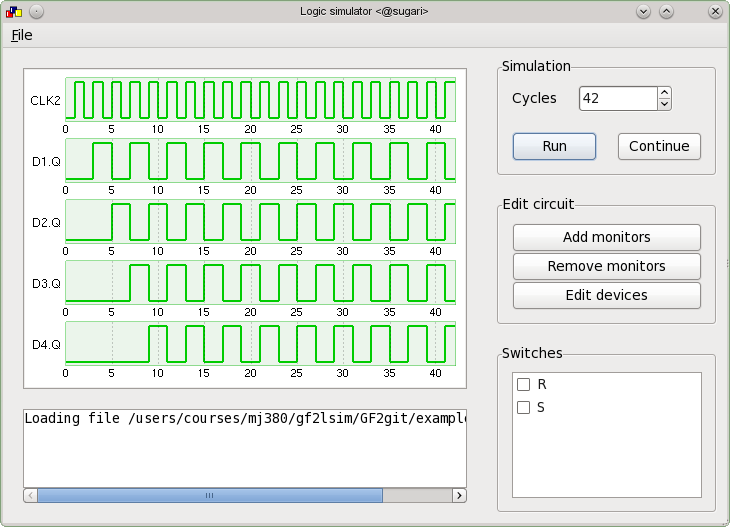
\includegraphics[width=16cm]{simulation.png}
 \caption{Main logic simulator window}
 \label{fig:gui-main}
\end{figure}
\begin{figure}[h]
 \centering
 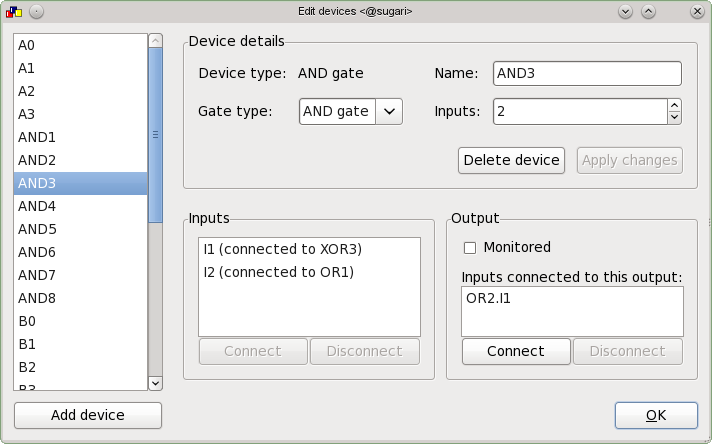
\includegraphics[width=16cm]{devices.png}
 \caption{GUI for editing devices}
 \label{fig:gui-devices}
\end{figure}

\clearpage
\section{Example circuits}
\label{sec:examples}
Jamie Magee made all definition files and circuit diagrams shown here.

\subsection{XOR Gate}
\subsubsection{Definition File}
\lstinputlisting[caption=xor.gf2]{../../examples/xor.gf2}
\subsubsection{Circuit Diagram}
\begin{figure}[h]
 \centering
 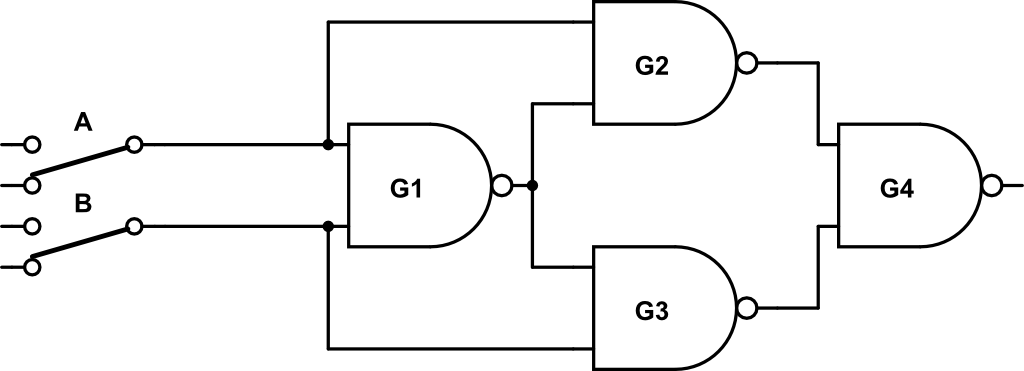
\includegraphics[width=8cm]{../../examples/xor.png}
 \caption{Circuit diagram of an XOR gate implemented using NAND gates}
 \label{fig:example-xor}
\end{figure}

\subsection{4-bit Adder}
\subsubsection{Definition File}
\lstinputlisting[caption=4bitadder.gf2]{../../examples/4bitadder.gf2}
\subsubsection{Circuit Diagram}
\begin{figure}[h]
 \centering
 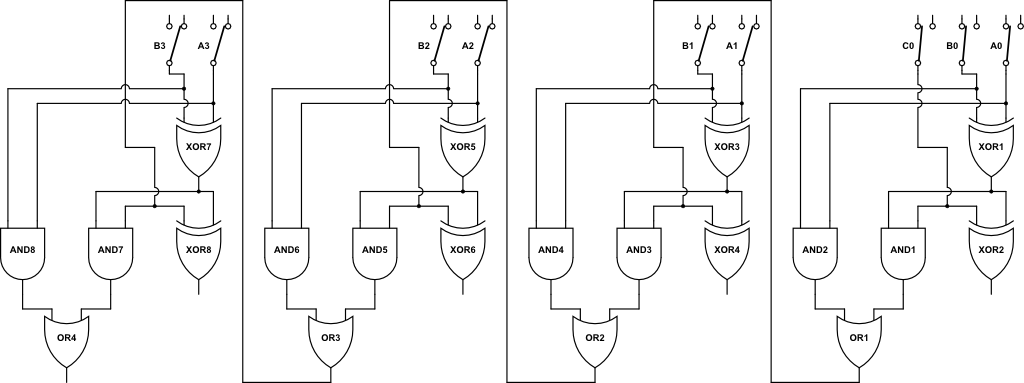
\includegraphics[width=16cm]{../../examples/4-bit-adder.png}
 \caption{Circuit diagram of a 4-bit adder}
 \label{fig:example-adder}
\end{figure}

\subsection{Serial In Parallel Out Shift Register}
\subsubsection{Definition File}
\lstinputlisting[caption=sipo.gf2]{../../examples/sipo.gf2}
\subsubsection{Circuit Diagram}

\begin{figure}[h]
 \centering
 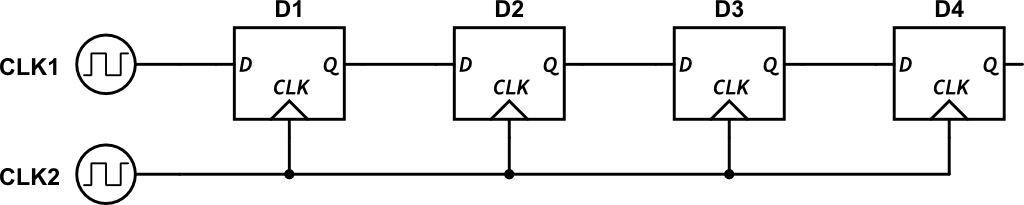
\includegraphics[width=12cm]{../../examples/sipo.png}
 \caption{Circuit diagram of a serial in parallel out shift register}
 \label{fig:example-sipo}
\end{figure}

\textbf{NB} The software used to draw the circuit diagram does not support the same style of D flip-flop used in the definition file, and Fig. \ref{fig:example-sipo} was the closest achievable.

\subsection{Gated D Latch}
\subsubsection{Definition File}
\lstinputlisting[caption=sipo.gf2]{../../examples/gateddlatch.gf2}
\subsubsection{Circuit Diagram}
\begin{figure}[h]
 \centering
 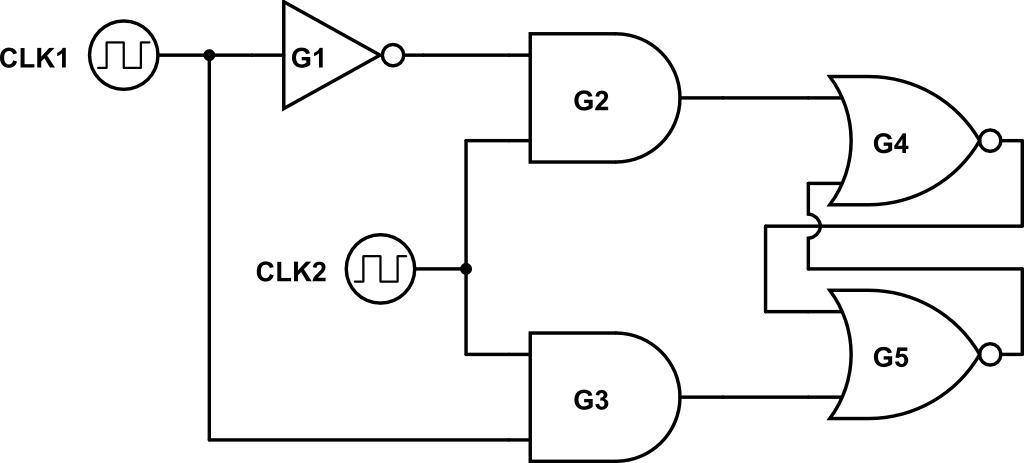
\includegraphics[width=12cm]{../../examples/gated-d-latch.png}
 \caption{Circuit diagram of a Gated D Latch}
 \label{fig:example-dlatch}
\end{figure}

\textbf{NB} The software used to draw the circuit diagram does not support NAND gates with one input. Therefore the NAND gate G1 was substituted for a NOT gate as can be seen in Fig. \ref{fig:example-dlatch}.


\end{document}


